\chapter{Heterogeneous Graphs}
\section{Heterogeneous Graph Definition}
A heterogeneous graph is defined as 
    \begin{align*}
        G = (V, E, R, T)
    \end{align*}
    \begin{itemize}
        \item Nodes with node type $v_i \in V$
        \item Edges with relation type $(v_i, r, v_j) \in E$
        \item Node Type $T(v_i)$
        \item Relation type $r\in R$
    \end{itemize}

\section{Relational GCN}
Extending to heterogeneous graph from the GCN by using different neural network weights for each relation type

\begin{align*}
    h_v^{(l+1)} = \sigma \left( \left(\sum_{r\in R} \sum_{u \in N(v)^r} \frac{1}{c_{v,r}} W_r^{(l)}h_u^{(l)}\right) + W_0^{(l)}h_v^{(l)} \right)
\end{align*}
    \begin{itemize}
        \item $c_{v,r}$ is the node degree of the given relationship
    \end{itemize}
But this way we have rapids growth in number of parameters w.r.t to number of relations. So overfitting become an issue. So we use the following two methods to regularize the weights $w_r^{(l)}$: 
    \begin{itemize}
        \item Use block diagonal matrices for neural network 
        \item Basis/Dictionary learning: Represent the matrix of each relation as a linear combination of basis transformations $W_r = \sum_{b=1}^B a_{rb} \cdot V_b$ where $V_b$ is shared across all relations. So now each relation only needs to learn $\{ a_{rb} \}$ which is B scalars and $V_b$ basis matrices which is B matrices. 
    \end{itemize}
    
\subsection{Link Prediction with GCN} 
For link prediction, now we need one prediction head for each type of relations since there could be multiple edge type. So assume $(E, r_3, A)$ is training supervision edge and all the other edges are training message edges. We need to 
    \begin{itemize}
        \item Take the final layer of $E$ and $A$: $h_E^{(l)}$ and $h_A^{(l)} \in \mathbbm{R}^d$ and relation-specific scoring function (one function per relationship). E.g.: $f_{r_1} = h_E^T W_{r_1}h_A$
        \item Here $W_{r_1}$ is a new matrix specifically for getting the relation specific scoring. 
    \end{itemize}
\begin{figure}[h]
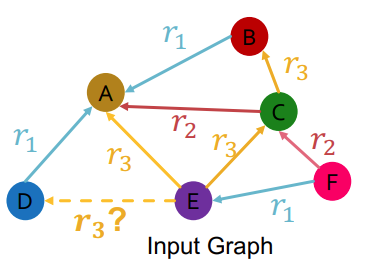
\includegraphics[width=6cm, height=6cm]{images/004_RGCN_example.png}
\end{figure}
In practice, we 
    \begin{enumerate}
        \item Use RGCN to score the training supervision edge $(E, r_3, A)$
        \item Create negative edge by pertubing the supervision edges. e.g.: $(E,r_3,B)$ if $E$ and $B$ are not connected in real graph. Note that the negative edges should not belong to training message edges or training supervision edges. 
        \item Use GNN model to score negative edge 
        \item Optimize a standard cross entropy loss (Maximize the score of training supervision edge and minimize the score of negative edge).
    \end{enumerate}
At evaluation time, let's say our target validation edge is $(E, r_3, D)$
    \begin{enumerate}
        \item Calculate the score of $(E, r_3, D)$
        \item Calculate the score of all the negative edges $(E, r_3, v)|v\in (B,F)$ since $(E,r_3,A)$ and $(E,r_3,C)$ belong to training message edges and training supervision edges. 
        \item Obtain the rank of $(E,r_3,D)$ We use rank because the result will be highly imbalanced class due to negative sampling
        \item Calculate metrics: 1)Hits at k : $\mathbbm{I}(RK \leq k )$, higher is better. 2): Reciprocal Rank $\frac{1}{RK}$, higher is better 
    \end{enumerate}
    
\section{Knowledge Graph: Predict Missing Tails}
Given an enormous knowledge graph, and a head and relation, we want to predict missing tails. Edges in KG are represented as triples $(h, r, t)$. The key idea is to model entities and relations in the embedding space $\mathbbm{R}^d$. So we want to make the embedding of $(h, r)$ to be close to the embedding of $t$

\subsection{Relation Type} 
Relations can be Symmetric, Inverse, Composition (Transitive) and 1 to N 

\subsection{TranSE} 
Intuition: For a triple $(h, r, t), h, r, t \in \mathbbm{R}^d$, we want $h + r \approx t$ if the given fact is true. The scoring function is $f_r(h,t) = - \norm{h + r - t }$. It cannot model symmetric and 1-to-N relations

\begin{figure}[H]
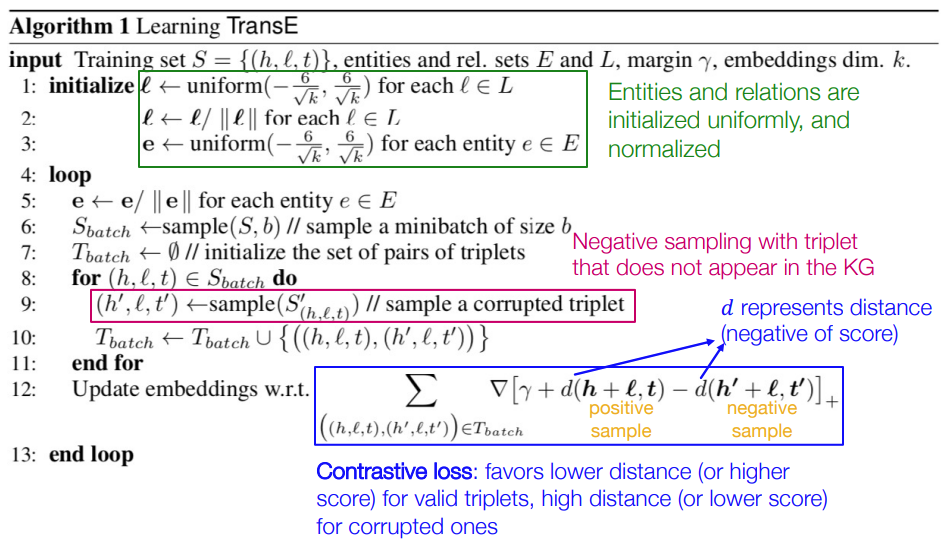
\includegraphics[width=12cm, height=9cm]{images/005_TransE.png}
\end{figure}

\subsection{TranR} 
Model entities as vectors in the entity space $\mathbbm{R}^d$ and model each relation as vector in relation space $r\in \mathbbm{R}^k$ with $M_r \in \mathbbm{R}^{k \times d}$ as the projection matrix that can transform entity to relation space.  So the scoring function is $f_r(h,t) = - \norm{M_rh + r - M_rt}$. It can model symmetric, antisymmetric, 1-to-N relation and inverse relationships. But it can not model transitive relations. 

\subsection{Bilinear Modeling} 
Entities and relations using vector in $\mathbbm{R}^k$. The scoring function $f_r(h,t) = <h, r, t> = \sum_i h_i \cdot r_i \cdot t_i$. It can model 1-to-N relations, symmetric, but not anti-symmetric, transitive and inverse. 

\subsection{ComplEX} 
Based on the same scoring function as bilinear modeling, but emebds entities and relations in complex vector space $\mathbbm{C}^k$. So the scoring function is $f_r(h,t) = Re(\sum_i h_i \cdot r_i \cdot \bar{t_i})$. $\bar{t}_i$ is the complex conjugate. It can model antisymmetric, symmetric, inverse, 1-to-N but can not model transitive relation. 


\section{Knowledge Graph: Multi-hop queries}
Knowledge graph completion problems can be reformulated as answering one-hop queries. i.e.: is link $(h, r, t)$ exists in the KG is equivalent to is $t$ an answer to query $(h,r)$. In general, we can formulate an $n-$ hop path query as 
    \begin{align*}
        q = (v_a, (r_1, ..., r_ n))
    \end{align*}
    \begin{itemize}
        \item $v_a$ is an "anchor" entity
        \item The answer in graph $G$ is denoted by $[[q]]_G$
    \end{itemize}
The goal is to answer path-based queries over an incomplete knowledge graph. So we are implicitly doing graph completion. 

\subsection{Query2Box Intuition} 
Map queries into embedding space and reason in the embedding space. Query2Box embed query into a hyper-rectangle (box) in the Euclidean space, the answer nodes are enclosed in the box. \\

TransE translate $h$ to $r$ with score function $f_r(h,t)=-\norm{h+r-t}$. Another way to look at is that the query embedding $q = h + r$, and we want query embedding $q$ close to the answer embedding $t$. i.e.: $f_q(t) = -\norm{q-t}$. We can easily extend TransE to handle compositional relations, i.e.: multi-hop queries. \\

We can embed queries with hyper-rectangles with a center and offset: $q = (Center(q), Offset(q))$. In this formulation, the intersection of boxes is well-defined (another box). So we can handle "and" logic. 


\subsection{Query2Box Embedding Details} 
For Query2Box, we need to figure out the following embedding / operations: 
    \begin{itemize}
        \item Entity embeddings (zero-volume box)
        \item Relation embeddings (take a box and produces a new box)
        \item Intersection operator $f$ (take multiple boxes and output a box). 
    \end{itemize}
    
\subsubsection{Relation Embeddings with Projection Operator} 
We can model relation embeddings with projection operator. It takes the current box as input and project and expand the box with a new center and offset. 

\subsubsection{Intersection Operator} 
Geometric intersection operator $j$ can be defined as 
    \begin{align*}
        & Cen(q_{inter}) = \sum_i w_i \odot Cen(q_i)\\
        & w_i = \frac{\exp(f_{cen}(Cen(q_i)))}{\sum_j \exp(f_cen(Cen(q_j)))}\\
        & Off(q_{inter}) = min(off(q_1),...,off(q_n)) \odot \sigma(f_{off}(off(q_1), ..., off(q_n)))
    \end{align*}
Where $w_i$ is calculated by a neural network $f_{cen}$. The offset is also calculated with neural network with sigmoid function 

\subsubsection{Entity-to-Box Distance} 
Given a query box $q$ and entity embedding box $v$, we can define the distance (L1 Distance) as 
    \begin{align*}
        & d_{box}(q,v) = d_{out}(q,v) + \alpha * d_{in}(q,v) & 0 < \alpha < 1
    \end{align*}
So we let the distance in the box to be down weighted. Finally we let the score $f_q(v) = -d_{box}(q,v)$

\subsubsection{Dealing with Union Operation} 
Since the union of boxes is not box. We can not establish a simple union operator. But we can take all the unions out and only do union at the last step (outside the embedding space). \\

In this way, the distance between query and an entity when dealing with "or" logic can be defined as 
    \begin{align*}
        & q = q_1 \vee q_2 \vee ... \vee q_m 
        & d_{box}(q,v) = min(d_{box}(q_1,v), ..., d_{box}(q_m,v))
    \end{align*}
Here each $q_i$ is a multi-hop query that does not contain "or" logic. 


\subsection{Training Query2Box}
Given a query embedding $q$, we want to maximzie the score $f_q(v)$ for answers $v \in [[q]]$ and minimize the score $f_q(v')$ for negative answers $v' \notin [[q]]$. The trainable parameters are : 
    \begin{itemize}
        \item Entity embeddings $d|v|$ (d dimension vector times vertiecs)
        \item relation embeddings $2d|R|$ (one set for move the center, one set for scale the box) 
        \item intersection operator 
    \end{itemize}
So the overall training summary is : 
    \begin{itemize}
        \item Randomly sample a query $q$ from the training graph $G_{train}$, answer $v\in [[q]]_{G_{train}}$ and negative sample $v' \notin [[q]]_{G_{train}}$. Negative sample has to have the same entity type as the positive answer. 
        \item Embed the query $q$
        \item Calculate the score $f_q(v)$ and $f_q(v')$
        \item Optimize the loss $l$ to maximize $f_q(v)$ while minimize $f_q(v')$. i.e.: $l = -\log \sigma(f_q(v)) - \log(1-\sigma(f_q(v')))$
    \end{itemize}
For the queries, we can sample them from a query template. We normally start with the answer and query template to find the anchor nodes. (Check lecture slides for detail). 